\subsubsection{Weighted case} \label{subsubsec:weighted}

The framework described above for the computation of eccentricities can be generalized to a more general kind of instance, made up of a median graph $G$ and a weight function $\alpha : V \rightarrow \mathbb{N}$. The \textit{weighted distance} $d_{\alpha}(u,v)$ is defined as the classical definition of the distance in addition with the weight of $v$: $d_{\alpha}(u,v) = d(u,v) + \alpha(v)$. Observe that the weighted distance is not symmetric anymore, as $\alpha(u)$ and $\alpha(v)$ may not be equal. The notions of shortest paths and intervals however remain the same than in the unweighted case.

We naturally extend the definition of labels $\varphi(u,L)$ to their weighted version $\varphi_{\alpha}(u,L)$. Let $\varphi_{\alpha}(u,L)$ be the maximum weighted distance $d_{\alpha}(u,v)$ such that $u \in I(v_0,v)$ and $L_{u,v} = L$. Let $u^+$ be the anti-basis of the hypercube with basis $u$ and signature $L$. Either $u^+$ is the vertex $v$ maximizing $\varphi_{\alpha}(u,L)$: in this case, $\varphi_{\alpha}(u,L) = \card{L} + \alpha(v)$. Otherwise, $v \neq u^+$ and $\varphi_{\alpha}(u,L)$ can be determined with an inductive formula, as stated in Equation~\eqref{eq:induction_phi}.

\[
    \varphi_{\alpha}(u,L) = \max\limits_{\substack{L^+ ~\mbox{\scriptsize{POF outgoing from}}~ u^+ \\ \forall E_j \in L^+,~ L \cup \set{E_j} ~\mbox{\scriptsize{not POF}}}} (\card{L} + \varphi_{\alpha}(u^+,L^+)).
\]

Taking the maximum value obtained between the two cases provide us with the correct $\varphi_{\alpha}(u,L)$. One can see that $\varphi$-labelings are the key concept of the algorithm evoked by Theorem~\ref{th:simple_ecc}. Indeed, the computation of labels $\opp$ and $\psi$ depend on labels $\varphi$. 

Label $\opp_{u,\alpha}(L)$ is defined as a POF $L'$ disjoint from $L$ maximizing $\varphi_{\alpha}(u,L')$. Theorem~\ref{th:compute_opp} is naturally generalized to the weighted case by considering, for the star graph $G_u$, the weights $\omega_u(L) = \varphi_{\alpha}(u,L)$ instead of $\varphi(u,L)$.

Label $\psi_{\alpha}(u,R)$ is defined as the maximum distance $d_{\alpha}(u,v)$ with a vertex $v$ such that $m(u,v,v_0) \neq u$ and the anti-ladder set of $m,u$ is $R$. Let $u^-$ be the basis of hypercube with anti-basis $u$ and signature $R$. Either $m = u^-$ and the anti-ladder label can be written as $\psi_{\alpha}(u,R) = \card{R} + \varphi_{\alpha}(u^-,\opp_{u^-,C}(R))$. Otherwise, it can be expressed as in inductive formula, as stated in Equation~\eqref{eq:induction_psi}.

\[
\psi_{\alpha}(u,R) = \max\limits_{\substack{R^- ~\mbox{\scriptsize{POF ingoing to}}~ u^- \\ \forall E_j \in R, R^- \cup \set{E_j} ~\mbox{\scriptsize{not POF}}}} (\card{R} + \psi_{\alpha}(u^-,R^-))
\]

Figure~\ref{fig:weights} illustrates the weighted labels $\varphi_{\alpha}$ and $\psi_{\alpha}$. It gives a median graph, two vertices $u$ and $v$, a POF $L$ outgoing from $u$ and a POF $R$ ingoing into $v$. Some vertices $x \in V$ are indexed with their weight $\alpha(x)$. The vertices with no index have weight 0. The reader can check the values provided for the different weighted and unweighted labels.

In brief, all labels $\varphi_{\alpha}$, $\opp_{u,\alpha}$, and $\psi_{\alpha}$ of a weighted median graph can be determined in $\tilde{O}(2^{2d}n)$. The \textit{weighted eccentricity} $\ecc_{\alpha}(u)$ of a vertex $u$ is naturally defined as the maximum distance $d_{\alpha}(u,v)$. Either the median $m = m(u,v,v_0)$ is $u$ and, hence, $\ecc_{\alpha}(u)$ is necessarily a label $\varphi_{\alpha}(u,L)$. Otherwise, set $\Pi(m,u)$ contains at least two elements and $d_{\alpha}(u,v)$ can be expressed as a label $\psi_{\alpha}(u,R)$. This corresponds to the weighted version of Equation~\eqref{eq:ecc_labels}. In summary, all weighted eccentricities on weighted median graphs can also be computed in time $\tilde{O}(2^{2d}n)$.

\begin{figure}[t]
\centering
\scalebox{0.9}{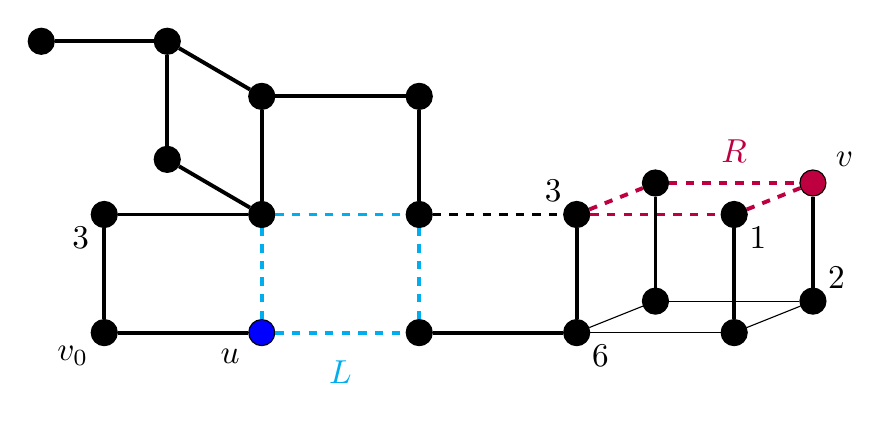
\begin{tikzpicture}

% NODES %%%%%%%%%%%%%%%%%%%%%%%%%%%%%%%%%%%%%%%%%%%%%%%%%%%%%%%%%%%%%%%%%%

\node[draw, circle, minimum height=0.2cm, minimum width=0.2cm, fill=black] (P11) at (1,1) {};
\node[draw, circle, minimum height=0.2cm, minimum width=0.2cm, fill=black] (P12) at (1,2.5) {};
\node[draw, circle, minimum height=0.2cm, minimum width=0.2cm, fill=black] (P13) at (0.2,4.7) {};

\node[draw, circle, minimum height=0.2cm, minimum width=0.2cm, fill=blue] (P21) at (3,1) {};
\node[draw, circle, minimum height=0.2cm, minimum width=0.2cm, fill=black] (P22) at (3,2.5) {};
\node[draw, circle, minimum height=0.2cm, minimum width=0.2cm, fill=black] (P23) at (3,4) {};
\node[draw, circle, minimum height=0.2cm, minimum width=0.2cm, fill=black] (P24) at (1.8,3.2) {};
\node[draw, circle, minimum height=0.2cm, minimum width=0.2cm, fill=black] (P25) at (1.8,4.7) {};

\node[draw, circle, minimum height=0.2cm, minimum width=0.2cm, fill=black] (P31) at (5,1) {};
\node[draw, circle, minimum height=0.2cm, minimum width=0.2cm, fill=black] (P32) at (5,2.5) {};
\node[draw, circle, minimum height=0.2cm, minimum width=0.2cm, fill=black] (P33) at (5,4) {};

\node[draw, circle, minimum height=0.2cm, minimum width=0.2cm, fill=black] (P41) at (7,1) {};
\node[draw, circle, minimum height=0.2cm, minimum width=0.2cm, fill=black] (P42) at (7,2.5) {};

\node[draw, circle, minimum height=0.2cm, minimum width=0.2cm, fill=black] (P51) at (9,1) {};
\node[draw, circle, minimum height=0.2cm, minimum width=0.2cm, fill=black] (P52) at (9,2.5) {};

\node[draw, circle, minimum height=0.2cm, minimum width=0.2cm, fill=black] (P61) at (8.0,1.4) {};
\node[draw, circle, minimum height=0.2cm, minimum width=0.2cm, fill=black] (P62) at (8.0,2.9) {};
\node[draw, circle, minimum height=0.2cm, minimum width=0.2cm, fill=black] (P63) at (10.0,1.4) {};
\node[draw, circle, minimum height=0.2cm, minimum width=0.2cm, fill=purple] (P64) at (10.0,2.9) {};


% LINKS %%%%%%%%%%%%%%%%%%%%%%%%%%%%%%%%%%%%%%%%%%%%%%%%%%%%%%%%%%%%%%%%%%


\draw[line width = 1.4pt] (P11) -- (P12);
\draw[line width = 1.4pt] (P11) -- (P21);
\draw[line width = 1.4pt] (P12) -- (P22);
\draw[line width = 1.4pt,dashed,color = cyan] (P21) -- (P22);

\draw[line width = 1.4pt,dashed,color = cyan] (P21) -- (P31);
\draw[line width = 1.4pt,dashed,color = cyan] (P22) -- (P32);
\draw[line width = 1.4pt,dashed,color = cyan] (P31) -- (P32);

\draw[line width = 1.4pt] (P22) -- (P23);
\draw[line width = 1.4pt] (P23) -- (P33);
\draw[line width = 1.4pt] (P32) -- (P33);

\draw[line width = 1.4pt] (P22) -- (P24);
\draw[line width = 1.4pt] (P23) -- (P25);
\draw[line width = 1.4pt] (P24) -- (P25);
\draw[line width = 1.4pt] (P13) -- (P25);

\draw[line width = 1.4pt] (P31) -- (P41);
\draw[line width = 1.4pt, dashed] (P32) -- (P42);
\draw[line width = 1.4pt] (P41) -- (P42);

\draw (P41) -- (P51);
\draw[line width = 1.4pt, dashed, color = purple] (P42) -- (P52);
\draw[line width = 1.4pt] (P51) -- (P52);

\draw (P41) -- (P61);
\draw[line width = 1.4pt, dashed, color = purple] (P42) -- (P62);
\draw (P51) -- (P63);
\draw[line width = 1.4pt, dashed, color = purple] (P52) -- (P64);
\draw[line width = 1.4pt] (P61) -- (P62);
\draw (P61) -- (P63);
\draw[line width = 1.4pt, dashed, color = purple] (P62) -- (P64);
\draw[line width = 1.4pt] (P63) -- (P64);


% ETIQUETTES

\node[scale=1.2, color = cyan] at (4.0,0.5) {$L$};
\node[scale=1.2, color = purple] at (9.0,3.3) {$R$};

\node[scale = 1.2] at (0.6,0.7) {$v_0$};
\node[scale = 1.2] at (2.6,0.7) {$u$};
\node[scale = 1.2] at (10.4,3.2) {$v$};

\node[scale = 1.2] at (7.3,0.7) {$6$};
\node[scale = 1.2] at (0.7,2.2) {$3$};
\node[scale = 1.2] at (9.3,2.2) {$1$};
\node[scale = 1.2] at (6.7,2.8) {$3$};
\node[scale = 1.2] at (10.3,1.7) {$2$};

\end{tikzpicture}
}
\caption{Label values: $\varphi(u,L) = 5 =d(u,v)$, $\varphi_{\alpha}(u,L) = 6$, $\psi(v,R) = 7$, $\psi_{\alpha}(v,R)= 8$.}
\label{fig:weights}
\end{figure}